\section{RNN}
Una TS è una \textbf{sequenza} di dati dispegata nel tempo. I dati sono tra loro correlati, quindi per una classica rete neurale bisognerebbe creare un input layer di dimensione pari alla lunghezza della TS in modo tale che la rete si alleni su una time series alla volta.\\
Essendo che le TS non sono quasi mai tutte della stessa lunghezza, bisognerebbe definire una rete differente per ogni tipologie di TS. Inoltre, l'input layer crescerebbe troppo.\\
\\
Un'idea potrebbe essere quella di lanciare diverse istanze della medesima rete neurale affinché ciascuna operi su porzioni diverse della serie, per poi mettere insieme i risultati, riprendendo un po' l'idea di un ensemble. \\
Questa soluzione, per quanto semplice, non funziona bene con sequenze di dati, poiché i dati sono tra loro correlati nel tempo: ogni valore nel tempo $t$ è legato al valore nel tempo $t-1$. Con questa soluzione le reti si addestrano su sottosequenze indipendenti della stessa TS, perdendo le correlazioni esistenti.\\
\\
Una \textbf{rete neurale ricorrente} (Recurrent Neural Network, RNN) è in grado di tenere memoria della sottosequenza analizzata nel passato e di prendere decisioni in funzione di esse.\\
Una RNN usa l'output del layer ricorrente come input dello stesso per certo numero di volte. Tra una ripetizione e l'altra i pesi calcolati dall'algoritmo di training sono conservati, così da tenere la memoria della sottosequenza di dati visti precedentemente.\\
I pesi che evolvono nel tempo formano il cosiddetto \textit{hidden state}. Questa tecnica viene chiamata \textbf{parameter sharing}.\\
La dimensione del layer ricorrente è fissata e andrà a determinare, chiaramente, le dimensioni dell'input e dell'output, e corrisponderà alla dimensione della sottosequenza che si desidera analizzare ad ogni passo.
\begin{figure}[H]
	\centering
	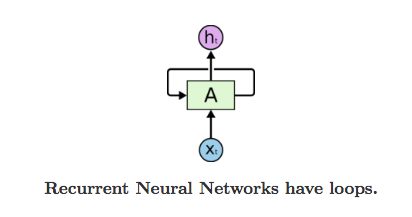
\includegraphics[width=\linewidth]{rnn.png}
	\caption{L'architettura base di una RNN}
	\label{fig:rnn}
\end{figure}
E' molto comune dare una rappresentazione \textit{unrolled} della rete per poterla ricondurre ad una rete neurale classica e comprenderne il funzionamento nel dettaglio.
\begin{figure}[H]
	\centering
	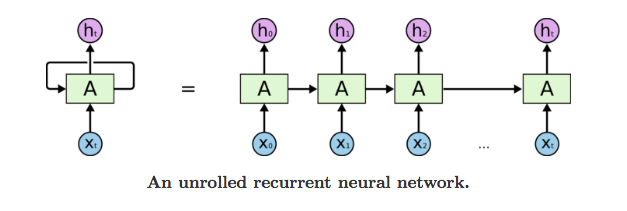
\includegraphics[width=\linewidth]{rnn_unrolled.png}
	\caption{La rappresentazione unrolled di una RNN}
	\label{fig:rnn_unrolled}
\end{figure}
Chiaramente, è possibile rendere più profonda una RNN, ed esistono diversi modi per farlo:
\begin{itemize}
	\item Aggiungere dei layer nascosti ricorrenti. Detta soluzione \textbf{stacked};
	\item Rendere il layer ricorrente una sotto-rete profonda;
	\item Aggiungere dei layer tra l'input e quello ricorrente;
	\item Aggiungere dei layer tra il ricorrente e l'output;
\end{itemize}

\subsection{LSTM}
Come evidenziato da bengio et al.\cite{long_term}, il modello standard di RNN nella pratica soffre di un problema long-term dependencies. Man mano che la rete compie un alto numero di ripetizioni del layer ricorrente, le caratteristiche apprese dalla prime ripetizioni iniziano a diventare meno rilevanti, quasi come se la rete iniziasse a dimenticare cosa ha fatto nel passato non recente. In alcuni casi è importante mantenere informazioni che risalgono ad un passato meno recente.\\
\\
Per risolvere questo problema, Hochreiter et al.\cite{lstm} hanno presentato la più applicata implementazione di RNN, ovvero le reti \textbf{LSTM, Long Short Term Memory}.\\
Il layer ricorrente di una LSTM segue una precisa struttura, ed è chiamato \textbf{cella LSTM}\footnote{I neuroni di una cella LSTM sono anche detti \textbf{unità LSTM}.}. Mentre nelle RNN standard i layer ricorrenti sono composti da neuroni che applicano una qualsiasi funzione di attivazione, un layer LSTM è invece composto da quattro sotto-layer, che applicano delle funzioni più complesse.
\begin{figure}[H]
	\centering
	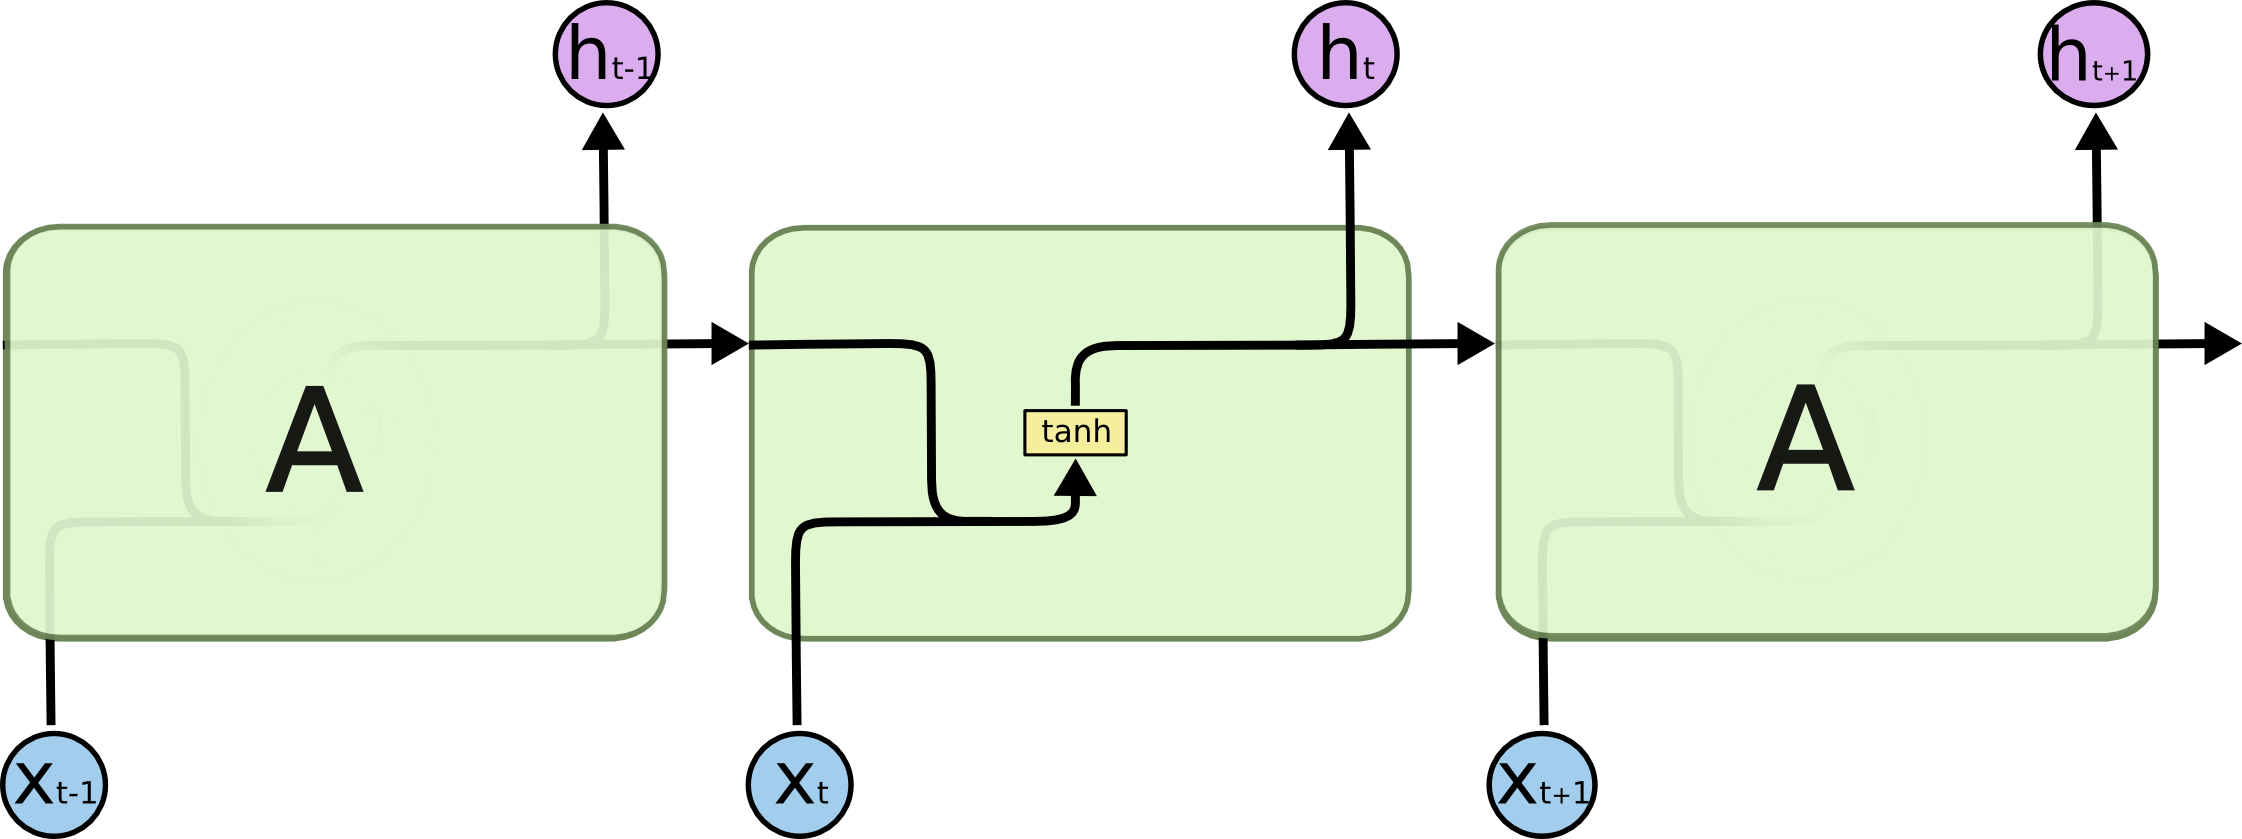
\includegraphics[width=\linewidth]{rnn_2.png}
	\caption{RNN unrolled standard. Nell'esempio viene usata la funzione di attivazione tangente iperbolica.}
	\label{fig:rnn_2}
\end{figure}
\begin{figure}[H]
	\centering
	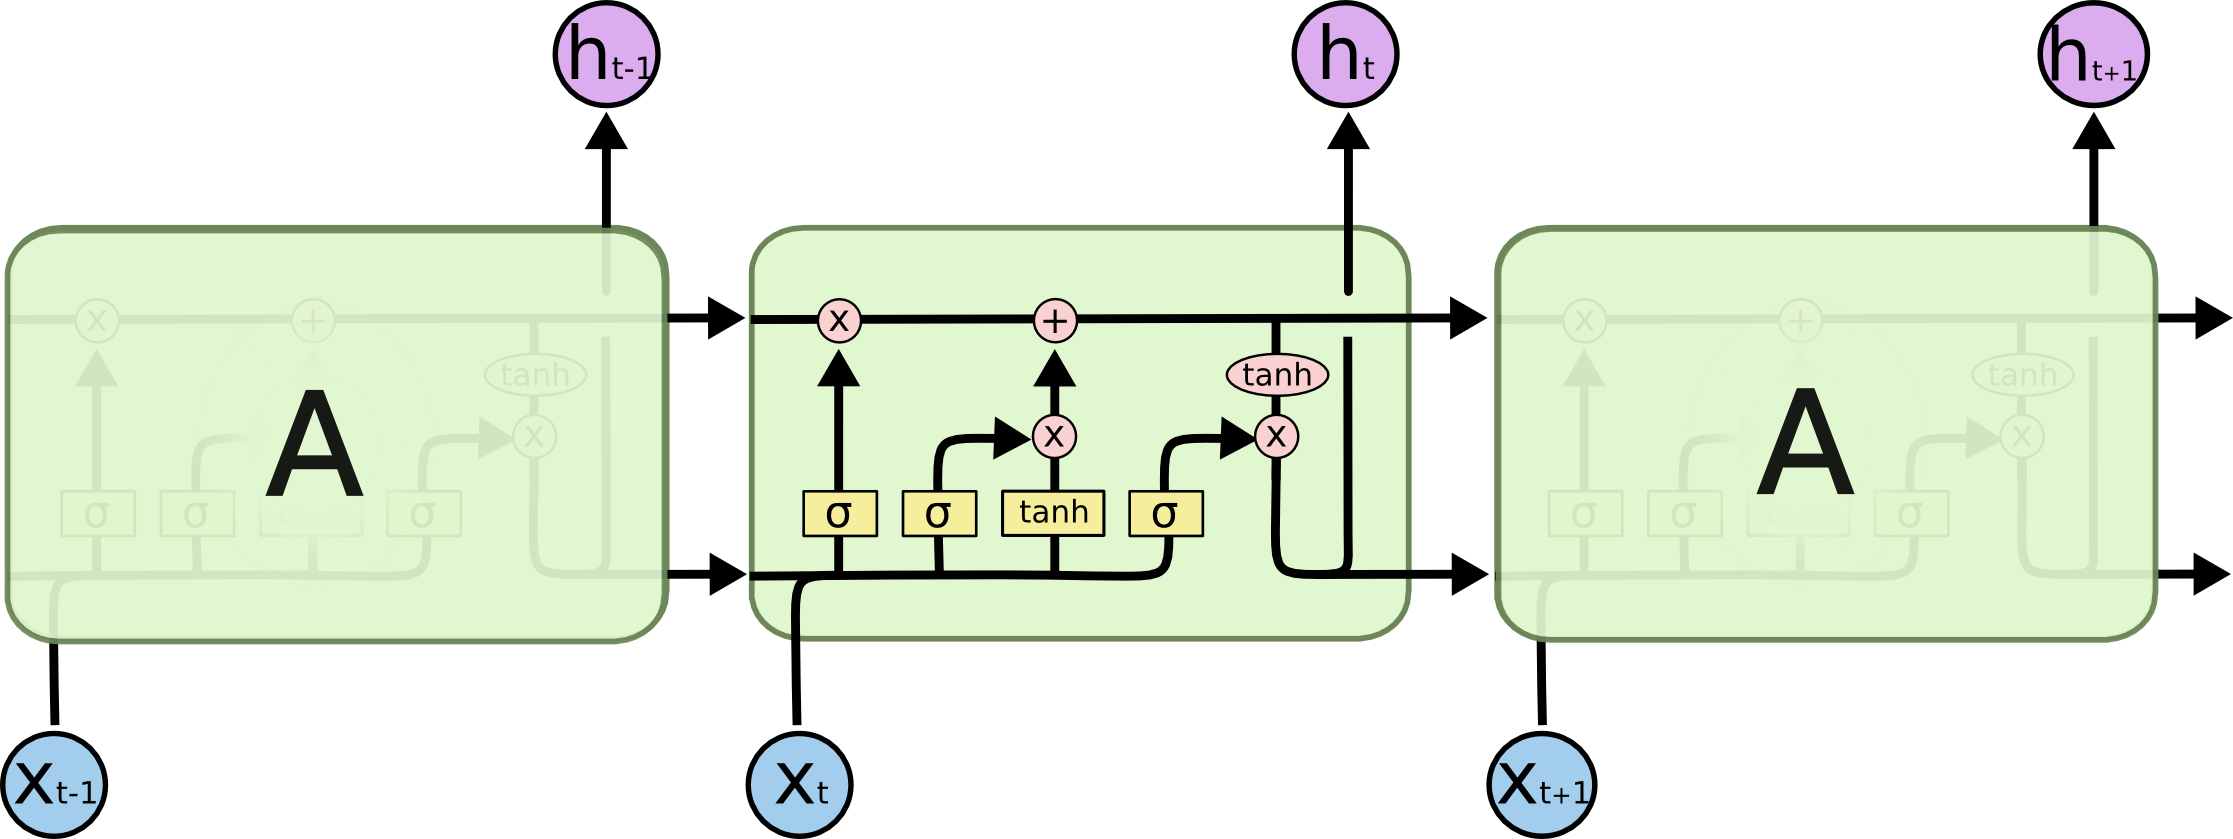
\includegraphics[width=\linewidth]{lstm.png}
	\caption{LSTM unrolled. I rettangoli gialli sono i quattro sotto-layer, di cui tre di essi applicano la semplice sigmoide, mentre l'altro la tangente iperbolica, mentre le figure rosa sono operazioni su vettori semplici.}
	\label{fig:lstm}
\end{figure}
La linea superiore della cella porta l'output superiore della cella precedente direttamente alla cella successiva, a meno di alcune operazioni lineari. Serve a mandare in avanti la conoscenza del passato senza modificarla troppo.\\
\\
La cella LSTM non segue necessariamente lo schema suddetto, ed esistono altre varianti, tutte accomunate dall'idea della linea superiore che preserva le long-term dependencies.

\section{Autoencoder}
Cos'è un autoencoder
Casi d'uso tipici

\section{Descrizione del modello proposto}
Perché lo abbiamo usato noi in questo caso
Struttura: stacked di 2 LSTM insomma, sia per encoder che per decoder
Come lo abbiamo usato (setting iperparametri, cosa abbiamo preso da esso (i vettori latenti) e cosa no)

\subsection{Training}
Come è stato allenato il modello (tensor flow e l'idea descritta con snippet notebook)

\section{Clustering con k-Means}
Come è stato lanciato k-means (su quali dati e con quali iperparametri)
Come è stato determinato il k, e per quali k abbiamo provato
Perché non si usa il DTW: i latent vector non sono TS!!

\subsection{Valutazione dei risultati}
Descrizione metriche, interne ed esterne, per ogni dataset
Osservazioni dei risultati (ad es. la purity è spesso alta, mentre un'altra cosa varia molto, o che su dataset grandi funziona bene, su piccoli no, ecc.): risultati da importare da file perché scriverli a mano è nu burdell.
-------------------------------------\\

Sia n il numero di classi di un dataset:
\begin{enumerate}[(i)]
	\item Se $n=2$, allora si esegue 2-Means, 3-Means e 4-Means;
	\item Se $n>2$, allora si esegue n-1-Means, n-Means ed n+1-Means.
\end{enumerate}

Di seguito sono riportati i risultati del clustering di alcuni dei dataset scelti.
\begin{table}[H]
	\centering
	\begin{tabularx}{\textwidth}{X | c c c c}
		\hline
		\textbf{Name} & \textbf{\#clusters} & \textbf{Silhouette} & \textbf{DB} & \textbf{Dunn} \\
		\hline
		\textbf{ECG5000} & 4 & \textbf{0.299} & \textbf{1.583} & / \\
		& 5 & 0.184 & 1.915 & / \\
		& 6 & 0.174 & 1.748 & / \\
		\hline
		\textbf{ECG200} & 2 & 0.220 & 1.215 & / \\
		& 3 & \textbf{0.326} & \textbf{1.059} & / \\
		& 4 & 0.277 & 1.270 & / \\
		\hline
		\textbf{ChlorineConc.} & 2 & \textbf{0.437} & 0.970 & / \\
		& 3 & 0.394 & 0.990 & / \\
		& 4 & 0.389 & \textbf{0.892} & / \\
		\hline
		\textbf{FordA} & 2 & \textbf{0.02} & \textbf{6.873} & / \\
		& 3 & 0.005 & 9.193 & / \\
		& 4 & -0.001 & 10.972 & / \\
	\end{tabularx}
	\caption{Misure interne del clustering con 100 iterazioni}
	\label{tab:clustering100_int}
\end{table}

\begin{table}[H]
	\centering
	\begin{tabularx}{\textwidth}{X | c c c c c}
		\hline
		\textbf{Name} & \textbf{\#clusters} & \textbf{Purity} & \textbf{Rel. Purity} & \textbf{ARI} & \textbf{FM}\\
		\hline
		\textbf{ECG5000} & 4 & 0.885 & \textbf{0.692} & \textbf{0.494} & \textbf{0.690} \\
		& 5 & 0.888 & 0.526 & 0.395 & 0.614 \\
		& 6 & \textbf{0.920} & 0.606 & 0.409 & 0.623 \\
		\hline
		\textbf{ECG200} & 2 & 0.688 & 0.688 & 0.030 & \textbf{0.709} \\
		& 3 & \textbf{0.75} & \textbf{0.75} & \textbf{0.230} & 0.627 \\
		& 4 & \textbf{0.75} & \textbf{0.75} & 0.108 & 0.468 \\
		\hline
		\textbf{ChlorineConc.} & 2 & \textbf{0.533} & 0.25 & \textbf{-0.001} & \textbf{0.444} \\
		& 3 & \textbf{0.533} & 0.25 & \textbf{-0.001} & 0.380 \\
		& 4 & \textbf{0.533} & \textbf{0.341} & \textbf{-0.001} & 0.315 \\
		\hline
		\textbf{FordA} & 2 & 0.522 & 0.522 & \textbf{0.001} & \textbf{0.5} \\
		& 3 & \textbf{0.528} & \textbf{0.528} & \textbf{0.001} & 0.419 \\
		& 4 & \textbf{0.528} & \textbf{0.528} & \textbf{0.001} & 0.364 \\
	\end{tabularx}
	\caption{Misure esterne del clustering con 100 iterazioni}
	\label{tab:clustering100_ext}
\end{table}